\documentclass{article}
\usepackage[utf8]{inputenc}
% are all of these packages really necessary?
% no.
% i'm just too lazy to only grab the packages i want for a specific
% document, so i just glob all of my most commonly used packages together
% this is bad practice.
\usepackage{amsmath,amsthm,amssymb,amsfonts, fancyhdr, color, comment, graphicx, environ, mdframed, soul, calc, enumitem, mdframed, xcolor, geometry, empheq, mathtools, tikz, pgfplots, caption, subcaption, hyperref}

\usetikzlibrary{external}
\tikzexternalize[prefix=tikz/,optimize command away=\includepdf]

%tikzpicture
\usepackage{tikz}
\usepackage{scalerel}
\usepackage{pict2e}
\usepackage{tkz-euclide}
\usetikzlibrary{calc}
\usetikzlibrary{patterns,arrows.meta}
\usetikzlibrary{shadows}
\usetikzlibrary{external}

%pgfplots
\usepackage{pgfplots}
\pgfplotsset{compat=newest}
\usepgfplotslibrary{statistics}
\usepgfplotslibrary{fillbetween}
\usepgfplotslibrary{polar}

\tikzset{external/export=true}
\pgfplotsset{
    standard/.style={
    axis line style = thick,
    trig format=rad,
    enlargelimits,
    axis x line=middle,
    axis y line=middle,
    enlarge x limits=0.15,
    enlarge y limits=0.15,
    every axis x label/.style={at={(current axis.right of origin)},anchor=north west},
    every axis y label/.style={at={(current axis.above origin)},anchor=south east}
    }
}
\newcommand*\widefbox[1]{\fbox{\hspace{2em}#1\hspace{2em}}}
% Command "alignedbox{}{}" for a box within an align environment
% Source: http://www.latex-community.org/forum/viewtopic.php?f=46&t=8144
\newlength\dlf  % Define a new measure, dlf
\newcommand\alignedbox[2]{
% Argument #1 = before & if there were no box (lhs)
% Argument #2 = after & if there were no box (rhs)
&  % Alignment sign of the line
{
\settowidth\dlf{$\displaystyle #1$}  
    % The width of \dlf is the width of the lhs, with a displaystyle font
\addtolength\dlf{\fboxsep+\fboxrule}  
    % Add to it the distance to the box, and the width of the line of the box
\hspace{-\dlf}  
    % Move everything dlf units to the left, so that & #1 #2 is aligned under #1 & #2
\boxed{#1 #2}
    % Put a box around lhs and rhs
}
}

\hypersetup{
    colorlinks=true,
    linkcolor=blue,
    filecolor=magenta,      
    urlcolor=cyan,
    pdftitle={Homework 8 Solutions},
    pdfpagemode=UseOutlines,
    bookmarksopen=true,
    pdfauthor={Christina Phan}
}
\newcommand{\lrp}[1]{\left( #1 \right)}
\newcommand{\abs}[1]{\left\vert #1 \right\vert}
\newcommand{\lra}[1]{\left\langle #1 \right\rangle}
\newcommand{\lrb}[1]{\left[ #1 \right]}
\newcommand{\iintR}[0]{\iint\limits_{R}}

\geometry{letterpaper, portrait, margin=1in}
\renewcommand{\footrulewidth}{0.8pt}
\setlength\parindent{0pt}
\pagestyle{fancy}
\lhead{Christina Phan}
\rhead{MAT 21D} 
\chead{\textbf{Homework 8 Solutions}}

\newcommand{\Solution}{\textit{Solution}}
\pgfplotsset{compat=1.18}
\begin{document}
\textbf{Note}

Yes, these solutions are done in a round-a-bout way. The unit tangent vector can just be found from $\mathbf{r}'(t)$ and its magnitude alone since $s'(t)=\lVert\mathbf{r}'(t)\rVert$.

\phantomsection
\addcontentsline{toc}{section}{Problem 1 (Parts)}\textbf{Problem 1 (Parts)}

Find the unit tangent vector and the length of the indicated portion of the curve:

\phantomsection
\addcontentsline{toc}{subsection}{1(a)}\textbf{(a)} $\displaystyle \mathbf{r}(t)=\lra{6\sin2t,6\cos2t,5t}, 0\leq t\leq \pi$

\Solution

Recall that the unit tangent vector and length of a portion of a curve are
\begin{align*}
    T&=\frac{\mathbf{r}'(t)}{{s}'(t)}\\
    s(t)&=\int_{t_0}^t\lVert\mathbf{r}'(\tau)\rVert\,d\tau
\end{align*}
Let's solve for $\mathbf{r}'(t)$, $s(t)$, and $s'(t)$.
\begin{align*}
    \mathbf{r}'(t)&=\lra{12\cos 2t,-12\sin 2t, 5}\\
    s(t)&=\int_0^t \lVert \mathbf{r}'(\tau)\rVert\,d\tau\\
    &=\int_0^t \sqrt{(12\cos 2\tau)^2 + (-12\sin 2\tau)^2 + (5)^2}\,d\tau\\
    &=\int_0^t \sqrt{144\cos^2 2\tau + 144\sin^2 2\tau + 25}\,d\tau\\
    &=\int_0^t \sqrt{144 (\cos^2 2\tau + \sin^2 2\tau) + 25}\,d\tau\\
    &=\int_0^t \sqrt{144 + 25}\,d\tau \tag{$\sin^2 x+\cos^2 x = 1$}\\
    &=\int_0^t 13 \,d\tau \tag{$\sqrt{144+25}=\sqrt{169}=13$}\\
    &=\lrb{13\tau}_0^t\\
    &=13t\\
    s'(t)&=13
\end{align*}
Putting it all together, our unit tangent vector must be
\begin{align*}
    T&=\frac{\mathbf{r}'(t)}{{s}'(t)}=\frac{1}{13}\lra{12\cos 2t,-12\sin 2t, 5}
\end{align*}
At $t=\pi$,
\begin{align*}
    s(\pi)&=13(\pi)=13\pi
\end{align*}
Our final answer is
\begin{subequations}
    \begin{empheq}[box=\widefbox]{align}
         T(t)&=\frac{1}{13}\lra{12\cos 2t,-12\sin 2t, 5}\nonumber\\
         s(\pi)&=13\pi\nonumber
    \end{empheq}
\end{subequations}
\phantomsection
\addcontentsline{toc}{subsection}{1(b)}\textbf{(b)} $\displaystyle \mathbf{r}(t)=\lra{t,0,\frac{2}{3}t^{3/2}}, 0\leq t\leq 8$

\Solution

Recall that the unit tangent vector and length of a portion of a curve are
\begin{align*}
    T&=\frac{\mathbf{r}'(t)}{{s}'(t)}\\
    s(t)&=\int_{t_0}^t\lVert\mathbf{r}'(\tau)\rVert\,d\tau
\end{align*}
Let's solve for $\mathbf{r}'(t)$, $s(t)$, and $s'(t)$.
\begin{align*}
    \mathbf{r}'(t)&=\lra{1,0,t^{1/2}}\\
    s(t)&=\int_0^t \lVert \mathbf{r}'(\tau)\rVert\,d\tau\\
    &=\int_0^t \sqrt{(1)^2 +(0)^2 +(\tau^{1/2})^2}\,d\tau\\
    &=\int_0^t \sqrt{1 + \tau}\,d\tau\\
    &=\lrb{\frac{2}{3}(1+\tau)^{3/2}}_0^t\\
    &=\frac{2}{3}(1+t)^{3/2}-\frac{2}{3}\\
    s'(t)&=(1+t)^{1/2}
\end{align*}
Putting it all together, our unit tangent vector must be
\begin{align*}
    T&=\frac{\mathbf{r}'(t)}{{s}'(t)}=\frac{1}{(1+t)^{1/2}}\lra{1,0,t^{1/2}}
\end{align*}
At $t=8$,
\begin{align*}
    s(8)&=\frac{2}{3}(1+8)^{3/2}-\frac{2}{3}=\frac{52}{3}
\end{align*}
Our final answer is
\begin{subequations}
    \begin{empheq}[box=\widefbox]{align}
         T(t)&=\frac{1}{(1+t)^{1/2}}\lra{1,0,t^{1/2}}\nonumber\\
         s(8)&=\frac{52}{3}\nonumber
    \end{empheq}
\end{subequations}
\phantomsection
\addcontentsline{toc}{subsection}{1(c)}\textbf{(c)} $\displaystyle \mathbf{r}(t)=\lra{6t^3,-2t^3,-3t^3}, 1\leq t\leq 2$

\Solution

Recall that the unit tangent vector and length of a portion of a curve are
\begin{align*}
    T&=\frac{\mathbf{r}'(t)}{{s}'(t)}\\
    s'(t)&=\int_{t_0}^t\lVert\mathbf{r}'(\tau)\rVert\,d\tau
\end{align*}
Let's solve for $\mathbf{r}'(t)$, $s(t)$, and $s'(t)$.
\begin{align*}
    \mathbf{r}'(t)&=\lra{18t^2,-6t^2,-9t^2}\\
    s(t)&=\int_1^t \lVert \mathbf{r}'(\tau)\rVert\,d\tau\tag{we're starting at $t=1$!}\\
    &=\int_1^t \sqrt{(18\tau^2)^2+(-6\tau^2)^2+(-9\tau^2)^2}\,d\tau\\
    &=\int_1^t \sqrt{441\tau^2}\,d\tau\\
    &=\int_1^t 21\tau^2 \,d\tau\\
    &=\lrb{7\tau^3}_1^t\\
    &=7t^3-7\\
    s'(t)&=21t^2
\end{align*}
Putting it all together, our unit tangent vector must be
\begin{align*}
    T&=\frac{\mathbf{r}'(t)}{{s}'(t)}=\frac{1}{21t^2}\lra{18t^2,-6t^2,-9t^2}=\lra{\frac{6}{7},-\frac{2}{7},-\frac{3}{7}}
\end{align*}
At $t=2$,
\begin{align*}
    s(2)&=7(2)^3-7=49
\end{align*}
Our final answer is
\begin{subequations}
    \begin{empheq}[box=\widefbox]{align}
         T(t)&=\lra{\frac{6}{7},-\frac{2}{7},-\frac{3}{7}}\nonumber\\
         s(2)&=49\nonumber
    \end{empheq}
\end{subequations}
\phantomsection
\addcontentsline{toc}{section}{Problem 2 (Parts)}\textbf{Problem 2 (Parts)} 

Find the arc length parameter from the point $t = 0$ and the length of the indicated
portion of the curve:

\phantomsection
\addcontentsline{toc}{subsection}{2(a)}\textbf{(a)} $\displaystyle \mathbf{r}(t)=\lra{4\cos t,4\sin t, 3t},0\leq t\leq \frac{\pi}{2}$

\Solution

The arc length parameter from the point $t=0$ is
\begin{align*}
    s(t)=\int_0^{t}\lVert \mathbf{r}'(\tau)\rVert\,d\tau
\end{align*}
Let's find $\mathbf{r}'(t)$ and $s(t)$.
\begin{align*}
    \mathbf{r}'(t)&=\lra{-4\sin t, 4\cos t, 3}\\
    s(t)&=\int_0^t \sqrt{(-4\sin \tau)^2 + (4\cos \tau)^2 + (3)^2}\,d\tau\\
    &=\int_0^t \sqrt{16\sin^2\tau + 16\cos^2\tau + 9}\,d\tau\\
    &=\int_0^t \sqrt{16(\sin^2\tau + \cos^2\tau)+9}\,d\tau\\
    &=\int_0^t \sqrt{16+9}\,d\tau\tag{$\sin^2x +\cos^2x =1$}\\
    &=\int_0^t 5 \,d\tau\tag{$\sqrt{16+9}=\sqrt{25}=5$}\\
    &=\lrb{5\tau}_0^t\\
    &=5t
\end{align*}
For $0\leq t\leq \dfrac{\pi}{2}$,
\begin{align*}
    \text{length: }=s\lrp{\frac{\pi}{2}}-s(0)=5\lrp{\frac{\pi}{2}}-5(0)=\frac{5\pi}{2}
\end{align*}
Our final answer is
\begin{subequations}
    \begin{empheq}[box=\widefbox]{align}
        s(t)&=5t\nonumber\\
        \text{length:   }&\hspace{1em}\frac{5\pi}{2}\nonumber
    \end{empheq}
\end{subequations}
\phantomsection
\addcontentsline{toc}{subsection}{2(b)}\textbf{(b)} $\displaystyle \mathbf{r}(t)=\lra{e^t\cos t,e^t\sin t,e^t},-\ln 4\leq t\leq 0$

\Solution

The arc length parameter from the point $t=0$ is
\begin{align*}
    s(t)=\int_0^{t}\lVert \mathbf{r}'(\tau)\rVert\,d\tau
\end{align*}
Let's find $\mathbf{r}'(t)$ and $s(t)$.
\begin{align*}
    \mathbf{r}'(t)&=\lra{e^t\cos t - e^t\sin t, e^t\sin t + e^t\cos t, e^t}\\
    s(t)&=\int_0^t \sqrt{\lrp{e^{\tau}\cos\tau - e^\tau \sin \tau}^2+ \lrp{e^\tau\sin \tau + e^\tau\cos\tau}^2+\lrp{ e^\tau}^2}\,d\tau\\
    &=\int_0^t \sqrt{2e^{2\tau}\cos^2\tau +2e^{2\tau}\sin^2\tau + e^{2\tau}}\,d\tau\tag{msg me if you need this explained}\\
    &=\int_0^t\sqrt{2e^{2\tau}\lrp{\cos^2\tau + \sin^2\tau}+e^{2\tau}}\,d\tau\\
    &=\int_0^t \sqrt{
    2e^{2\tau}+e^{2\tau}}\,d\tau\tag{$\cos^2 x + \sin^2 x = 1$}\\
    &=\int_0^t e^\tau\sqrt{3}\,d\tau\tag{$\sqrt{2e^{2\tau}+e^{2\tau}}=\sqrt{3e^{2\tau}}=e^\tau\sqrt{3}$}\\
    &=\lrb{e^{\tau}\sqrt{3}}_0^t\\
    &=e^t\sqrt{3}- \sqrt{3}\tag{$e^0=1$}
\end{align*}
For $-\ln 4\leq t\leq 0$,
\begin{align*}
   \text{length} = s(0)-s(\ln 4)=\lrp{e^0\sqrt{3}-\sqrt{3}}-\lrp{e^{-\ln 4}\sqrt{3-\sqrt{3}}}=(0)-\lrp{\frac{1}{4}\sqrt{3}-\sqrt{3}}=\frac{3\sqrt{3}}{4}
\end{align*}
Our final answer is
\begin{subequations}
    \begin{empheq}[box=\widefbox]{align}
        s(t)&=e^t\sqrt{3}-\sqrt{3}\nonumber\\
        \text{length:   }&\hspace{1em}\frac{3\sqrt{3}}{4}\nonumber
    \end{empheq}
\end{subequations}
\phantomsection
\addcontentsline{toc}{section}{Problem 3}\textbf{Problem 3} 

In today’s lecture, we saw that the length of the helix $\mathbf{r}(t) =\lra{\cos t,\sin t,t}$ from
$t = 0$ to $t = 2\pi$ is $2\pi\sqrt{2}$. Show that it is possible to derive this result geometrically, as the diagonal of a square of side length $2\pi$.

\Solution

Imagine the helix $\mathbf{r}(t) =\lra{\cos t,\sin t,t}$ wrapping around a cylinder of radius $1$. Here's my amazing rendition of it. Alternatively, you can imagine this by taking a post-it note, drawing a diagonal line from corner to corner, and wrapping it into a cylinder by rolling the edges together.


\tikzset{every picture/.style={line width=0.75pt}} %set default line width to 0.75pt        

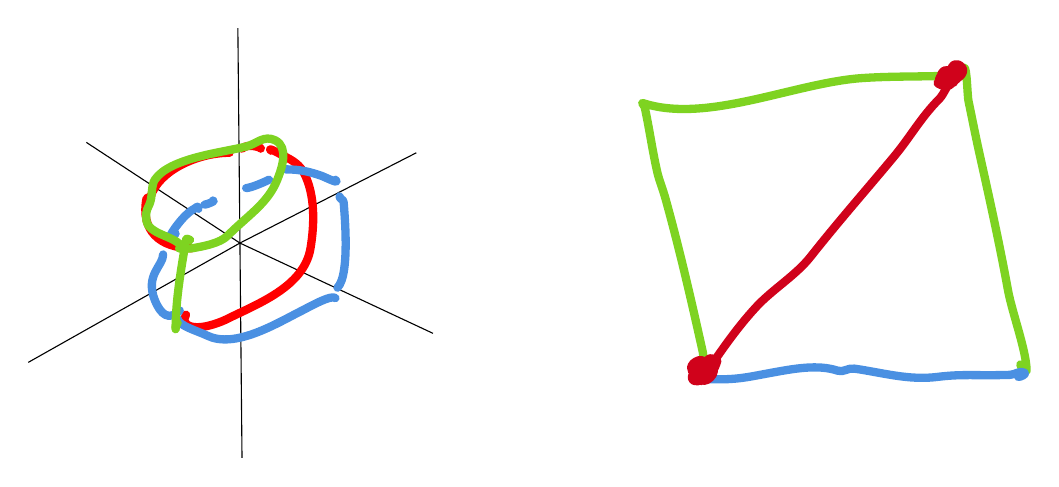
\begin{tikzpicture}[x=0.75pt,y=0.75pt,yscale=-1,xscale=1]
%uncomment if require: \path (0,300); %set diagram left start at 0, and has height of 300

%Straight Lines [id:da8494068874687858] 
\draw    (201,60.77) -- (203,267.77) ;
%Straight Lines [id:da1543256349566654] 
\draw    (202,164.27) -- (100,221.77) ;
%Straight Lines [id:da57810582099892] 
\draw    (202,164.27) -- (295,207.77) ;
%Straight Lines [id:da24462878338147642] 
\draw    (202,164.27) -- (287,120.77) ;
%Straight Lines [id:da9265264648869336] 
\draw    (202,164.27) -- (128,115.77) ;
%Shape: Free Drawing [id:dp7344388245144222] 
\draw  [color={rgb, 255:red, 255; green, 0; blue, 0 }  ,draw opacity=1 ][line width=3] [line join = round][line cap = round] (176,198.77) .. controls (176,200.44) and (174.61,200.99) .. (175,201.77) .. controls (178.06,207.89) and (190.85,203.34) .. (196,200.77) .. controls (210.51,193.51) and (232.9,185.35) .. (236,166.77) .. controls (237.99,154.83) and (238.21,141.19) .. (233,130.77) .. controls (230.96,126.68) and (227.53,124.53) .. (224,122.77) .. controls (222.18,121.86) and (214.76,117.53) .. (217,119.77) ;
%Shape: Free Drawing [id:dp698730010590395] 
\draw  [color={rgb, 255:red, 255; green, 0; blue, 0 }  ,draw opacity=1 ][line width=3] [line join = round][line cap = round] (212,118.77) .. controls (213.34,118.77) and (206.02,115.74) .. (203,118.77) ;
%Shape: Free Drawing [id:dp9961823220370511] 
\draw  [color={rgb, 255:red, 255; green, 0; blue, 0 }  ,draw opacity=1 ][line width=3] [line join = round][line cap = round] (197,120.77) .. controls (181.76,120.77) and (163.19,129.19) .. (159,141.77) .. controls (158.76,142.47) and (157.15,142.04) .. (157,142.77) .. controls (153.96,157.98) and (163.17,166.77) .. (179,166.77) ;
%Shape: Free Drawing [id:dp5844112483924738] 
\draw  [color={rgb, 255:red, 74; green, 144; blue, 226 }  ,draw opacity=1 ][line width=3] [line join = round][line cap = round] (172,200.77) .. controls (172,203.97) and (182.38,206.96) .. (186,208.77) .. controls (199.56,215.54) and (219.98,202.78) .. (232,196.77) .. controls (234.72,195.41) and (246.13,188.9) .. (248,190.77) ;
%Shape: Free Drawing [id:dp7253765541554063] 
\draw  [color={rgb, 255:red, 74; green, 144; blue, 226 }  ,draw opacity=1 ][line width=3] [line join = round][line cap = round] (249,185.77) .. controls (255.42,179.35) and (252.08,147.2) .. (252,144.77) .. controls (251.95,143.02) and (250,143.26) .. (250,141.77) ;
%Shape: Free Drawing [id:dp09668920319286944] 
\draw  [color={rgb, 255:red, 74; green, 144; blue, 226 }  ,draw opacity=1 ][line width=3] [line join = round][line cap = round] (248,133.77) .. controls (250.66,136.43) and (242.65,132.32) .. (241,131.77) .. controls (235.93,130.08) and (231.41,128.77) .. (224,128.77) ;
%Shape: Free Drawing [id:dp611131556590413] 
\draw  [color={rgb, 255:red, 74; green, 144; blue, 226 }  ,draw opacity=1 ][line width=3] [line join = round][line cap = round] (216,133.77) .. controls (213.67,134.93) and (207.16,137.77) .. (205,137.77) ;
%Shape: Free Drawing [id:dp10589312036494702] 
\draw  [color={rgb, 255:red, 74; green, 144; blue, 226 }  ,draw opacity=1 ][line width=3] [line join = round][line cap = round] (189,143.77) .. controls (191.01,143.77) and (185.85,145.77) .. (185,145.77) ;
%Shape: Free Drawing [id:dp48996324843934347] 
\draw  [color={rgb, 255:red, 74; green, 144; blue, 226 }  ,draw opacity=1 ][line width=3] [line join = round][line cap = round] (173,196.77) .. controls (167.86,201.91) and (163.83,198.85) .. (161,191.77) .. controls (156.13,179.59) and (165,175.3) .. (165,169.77) ;
%Shape: Free Drawing [id:dp9984471572612368] 
\draw  [color={rgb, 255:red, 74; green, 144; blue, 226 }  ,draw opacity=1 ][line width=3] [line join = round][line cap = round] (171,159.77) .. controls (163.38,167.38) and (173.31,151.11) .. (180,147.77) .. controls (180.77,147.38) and (182,145.71) .. (182,147.77) ;
%Shape: Free Drawing [id:dp07848402190455939] 
\draw  [color={rgb, 255:red, 126; green, 211; blue, 33 }  ,draw opacity=1 ][line width=3] [line join = round][line cap = round] (171,204.77) .. controls (171,204.77) and (171,204.77) .. (171,204.77) ;
%Shape: Free Drawing [id:dp27895987755991847] 
\draw  [color={rgb, 255:red, 126; green, 211; blue, 33 }  ,draw opacity=1 ][line width=3] [line join = round][line cap = round] (172,202.77) .. controls (170.95,202.77) and (171,206.82) .. (171,205.77) .. controls (171,191.63) and (173.74,176.34) .. (176,162.77) .. controls (176.21,161.5) and (177.27,162.77) .. (178,162.77) ;
%Shape: Free Drawing [id:dp6203777297952372] 
\draw  [color={rgb, 255:red, 126; green, 211; blue, 33 }  ,draw opacity=1 ][line width=3] [line join = round][line cap = round] (173,166.77) .. controls (170.94,166.77) and (176.54,167.18) .. (179,166.77) .. controls (183.78,165.97) and (192.28,164.49) .. (196,160.77) .. controls (206.17,150.6) and (215.43,145.18) .. (220,133.77) .. controls (222.15,128.39) and (225.73,118.13) .. (219,114.77) .. controls (213.56,112.05) and (210.06,116.5) .. (205,117.77) .. controls (193.49,120.64) and (168.01,123.25) .. (161,133.77) .. controls (159.36,136.22) and (159.73,140.85) .. (159,143.77) .. controls (157.95,147.97) and (156.13,147.65) .. (157,153.77) .. controls (157.81,159.44) and (169.25,161.02) .. (173,164.77) ;
%Shape: Free Drawing [id:dp470797652986484] 
\draw  [color={rgb, 255:red, 126; green, 211; blue, 33 }  ,draw opacity=1 ][line width=3] [line join = round][line cap = round] (427,224.77) .. controls (425.06,222.82) and (425.6,219.45) .. (425,216.77) .. controls (419.44,191.76) and (413.9,167.62) .. (407,142.77) .. controls (405.79,138.4) and (404,134.19) .. (403,129.77) .. controls (400.67,119.5) and (399.25,109.05) .. (397,98.77) .. controls (396.84,98.04) and (395.29,96.53) .. (396,96.77) .. controls (426.88,107.06) and (469.29,86.95) .. (502,84.77) .. controls (514.64,83.92) and (527.33,84.12) .. (540,83.77) .. controls (542.37,83.7) and (551,79.28) .. (551,83.77) ;
%Shape: Free Drawing [id:dp657810807193408] 
\draw  [color={rgb, 255:red, 126; green, 211; blue, 33 }  ,draw opacity=1 ][line width=3] [line join = round][line cap = round] (551,79.77) .. controls (552.28,79.77) and (552.45,93.13) .. (553,95.77) .. controls (554.68,103.76) and (556.23,111.79) .. (558,119.77) .. controls (562.94,142.01) and (567.92,164.35) .. (572,186.77) .. controls (574.02,197.86) and (581,216.3) .. (581,225.77) .. controls (581,227.18) and (578,224.18) .. (578,222.77) ;
%Shape: Free Drawing [id:dp7656865211840534] 
\draw  [color={rgb, 255:red, 74; green, 144; blue, 226 }  ,draw opacity=1 ][line width=3] [line join = round][line cap = round] (422,228.77) .. controls (420.95,228.77) and (423.95,229.72) .. (425,229.77) .. controls (441.04,230.41) and (445.23,229.09) .. (458,226.77) .. controls (468.94,224.78) and (480.5,222.6) .. (490,225.77) .. controls (492.88,226.73) and (494.73,224.3) .. (498,224.77) .. controls (511.57,226.71) and (524.15,230.5) .. (538,228.77) .. controls (550.37,227.22) and (556.97,228.3) .. (573,227.77) .. controls (575.36,227.69) and (578.04,225.46) .. (580,226.77) .. controls (581,227.43) and (578.2,228.77) .. (577,228.77) ;
%Shape: Free Drawing [id:dp2701440279466565] 
\draw  [color={rgb, 255:red, 208; green, 2; blue, 27 }  ,draw opacity=1 ][line width=3] [line join = round][line cap = round] (424,230.77) .. controls (432.12,218.58) and (441.17,205.25) .. (451,194.77) .. controls (458.83,186.41) and (469.89,179.78) .. (477,170.77) .. controls (490.06,154.23) and (503.65,138.79) .. (517,122.77) .. controls (524.96,113.22) and (530.13,103.64) .. (539,94.77) .. controls (541.84,91.93) and (542.99,85.77) .. (547,85.77) ;
%Shape: Free Drawing [id:dp2194482905818239] 
\draw  [color={rgb, 255:red, 208; green, 2; blue, 27 }  ,draw opacity=1 ][line width=3] [line join = round][line cap = round] (426,222.77) .. controls (432.13,222.77) and (423.34,225.84) .. (425,223.77) .. controls (426.59,221.78) and (432,218.23) .. (432,220.77) .. controls (432,221.39) and (429.05,230.84) .. (426,226.77) .. controls (424.73,225.07) and (426.41,219.77) .. (429,219.77) .. controls (433.51,219.77) and (427.51,229.97) .. (422,227.77) .. controls (418.11,226.21) and (418.64,222.22) .. (423,220.77) .. controls (428.73,218.86) and (426.57,232.62) .. (421,230.77) .. controls (416.83,229.38) and (424.04,220.79) .. (428,222.77) .. controls (434.93,226.23) and (424,234.28) .. (424,228.77) ;
%Shape: Free Drawing [id:dp4161028484602677] 
\draw  [color={rgb, 255:red, 208; green, 2; blue, 27 }  ,draw opacity=1 ][line width=3] [line join = round][line cap = round] (544,85.77) .. controls (548.75,85.77) and (544.33,88.42) .. (544,86.77) .. controls (543.52,84.38) and (544.76,76.65) .. (549,78.77) .. controls (551.87,80.2) and (546.22,85.42) .. (545,81.77) .. controls (543.85,78.33) and (547.54,76.48) .. (550,79.77) .. controls (552.04,82.49) and (546.61,86.64) .. (544,85.77) .. controls (540.21,84.5) and (544.7,79.88) .. (545,80.77) .. controls (546.07,83.98) and (541.09,88.03) .. (540,84.77) .. controls (538.97,81.67) and (542.67,78.88) .. (545,82.77) .. controls (547.28,86.56) and (540.17,90.28) .. (539,86.77) .. controls (537.76,83.04) and (543.97,80.64) .. (545,84.77) .. controls (546.8,91.97) and (534.72,86.77) .. (539,86.77) ;




\end{tikzpicture}

We have the radius be one since the maximum absolute value $x$ can be is $1$ and the maximum absolute value $y$ can be is $1$. The height of the cylinder would be $2\pi$ since $z$ goes from $0$ to $2\pi$.

If we unwrap the cylinder, we get a rectangle with a base of the circumference of the cylinder and height of $2\pi$. The path of the helix would go from the bottom corner of the rectangle to the top corner of the rectangle, diagonally. 

The circumference of the cylinder is $2\pi(1)=2\pi$.

Therefore, our rectangle is actually a square with side lengths of $2\pi$. The length of our helix is the diagonal (red line length) of the square with side length $2\pi$.

Using the Pythagorean Theorem,
\begin{align*}
    \text{length}&=\sqrt{(2\pi)^2+(2\pi)^2}=\sqrt{8\pi^2}=\boxed{2\pi\sqrt{2}}
\end{align*}
\phantomsection
\addcontentsline{toc}{section}{Problem 4}\textbf{Problem 4}

Consider a line $\mathbf{r}(t) = \lra{x_0,y_0}+ t\mathbf{u}$, where $\mathbf{u}$ is a unit vector. Show that the arc
length parameter $s$ along the line coincides with the time parameter $t$.

\Solution

The arc length parameter from the point $t=0$ is
\begin{align*}
    s(t)=\int_0^{t}\lVert \mathbf{r}'(\tau)\rVert\,d\tau
\end{align*}
Let's find $\mathbf{r}'(t)$ and $s(t)$.
\begin{align*}
    \mathbf{r}(t)&=\lra{x_0 + tu_1, y_0+tu_2}\\
    \mathbf{r}'(t)&=\lra{u_1,u_2}\tag{the other stuff is just constants}\\
    s(t)&=\int_0^t\lVert\mathbf{r}'(\tau)\rVert\,d\tau\\
    s(t)&=\int_0^t \sqrt{(u_1)^2+(u_2)^2}\,d\tau\\\
    &=\int_0^t \lVert \mathbf{u}\rVert\,d\tau\tag{def of magnitude}\\
    &=\int_0^t 1 \,d\tau\tag{$\mathbf{u}$ is a \textbf{unit} vector, so magnitude is $1$}\\
    &=\lrb{\tau}_0^t\\
    &=t
\end{align*}
Since $s(t)=t$, the arc length parameter $s$ along the line coincides with the time parameter $t$.\qed

\phantomsection
\addcontentsline{toc}{section}{Problem 5 (Parts)}\textbf{Problem 5}

Let $\mathbf{u}, \mathbf{v}, \mathbf{w}$, and $\mathbf{r}$ be differentiable vector-valued functions of $t$.

\phantomsection
\addcontentsline{toc}{subsection}{5(a)}
\textbf{(a)} Show that $\displaystyle\frac{d}{dt}\left(\mathbf{u}\cdot\mathbf{v}\times\mathbf{w}\right)=\mathbf{u}'\cdot\mathbf{v}\times\mathbf{w}+\mathbf{u}\cdot\mathbf{v}'\times\mathbf{w}+\mathbf{u}\cdot\mathbf{v}\times\mathbf{w}'$

\Solution

\begin{align*}
    \frac{d}{dt}\left(\mathbf{u}\cdot\mathbf{v}\times\mathbf{w}\right)&=\mathbf{u}'\cdot(\mathbf{v}\times\mathbf{w})+\mathbf{u}\cdot\frac{d}{dt}(\mathbf{v}\times\mathbf{w})\\
    &=\mathbf{u}'\cdot(\mathbf{v}\times\mathbf{w})+\mathbf{u}\cdot\left(\mathbf{v}'\times\mathbf{w}+\mathbf{v}+\mathbf{w}'\right)\\
    &=\mathbf{u}'\cdot\mathbf{v}\times\mathbf{w}+\mathbf{u}\cdot\mathbf{v}'\times\mathbf{w}+\mathbf{u}\cdot\mathbf{v}\times\mathbf{w}'
\end{align*}\qed

\phantomsection
\addcontentsline{toc}{subsection}{5(b)}
\textbf{(b)} Use this to show that $\displaystyle\frac{d}{dt}\left(\mathbf{r}\cdot\mathbf{r}'\times\mathbf{r}''\right)=\mathbf{r}\cdot\mathbf{r}'\times\mathbf{r}'''$.

\Solution

Since $\displaystyle\frac{d}{dt}\left(\mathbf{u}\cdot\mathbf{v}\times\mathbf{w}\right)=\mathbf{u}'\cdot\mathbf{v}\times\mathbf{w}+\mathbf{u}\cdot\mathbf{v}'\times\mathbf{w}+\mathbf{u}\cdot\mathbf{v}\times\mathbf{w}'$,
\begin{align*}
    \frac{d}{dt}\left(\mathbf{r}\cdot\mathbf{r}'\times\mathbf{r}''\right)&=\mathbf{r}'\cdot\mathbf{r}'\times\mathbf{r}''+\mathbf{r}\cdot\mathbf{r}''\times\mathbf{r}''+\mathbf{r}\cdot\mathbf{r}'\times\mathbf{r}'''\tag{plug n chug}
\end{align*}
We know that the dot product of orthogonal vectors is $0$ and that the cross product of parallel vectors is $0$. 

Putting this in the context of our problem, 

$\mathbf{r}'\times\mathbf{r}''$ is a cross product that is a vector that is \textit{perpendicular} to $\mathbf{r}'$. Again, the dot product of orthogonal vectors is $0$, so $\mathbf{r}'\cdot(\mathbf{r}'\times\mathbf{r}'')$ must equal $0$.

Clearly $\mathbf{r}''$ and $\mathbf{r}''$ are parallel to each other, so $\mathbf{r}''\times\mathbf{r}''$ must equal $0$ since the cross product of parallel vectors is $0$. Therefore, $\mathbf{r}\cdot\mathbf{r}''\times\mathbf{r}''=\mathbf{r}\cdot0=0$.

Putting this all together, we get
\begin{align*}
    \frac{d}{dt}\left(\mathbf{r}\cdot\mathbf{r}'\times\mathbf{r}''\right)&=\mathbf{r}'\cdot\mathbf{r}'\times\mathbf{r}''+\mathbf{r}\cdot\mathbf{r}''\times\mathbf{r}''+\mathbf{r}\cdot\mathbf{r}'\times\mathbf{r}'''\\
    &=0+0+\mathbf{r}\cdot\mathbf{r}'\times\mathbf{r}'''\\
    &=\boxed{\mathbf{r}\cdot\mathbf{r}'\times\mathbf{r}'''}
\end{align*}\qed
\end{document}
